\documentclass{article}

\usepackage[letterpaper,
	bindingoffset = 0in,
	left = 1in,
	right = 1in,
	bottom = 1in,
	top = 1in]{geometry}
\usepackage{caption}
\usepackage{float}
\usepackage{graphicx}

% supplementary prefix
\renewcommand{\thefigure}{S\arabic{figure}}

\begin{document}

\begin{figure}[h!]
\centering
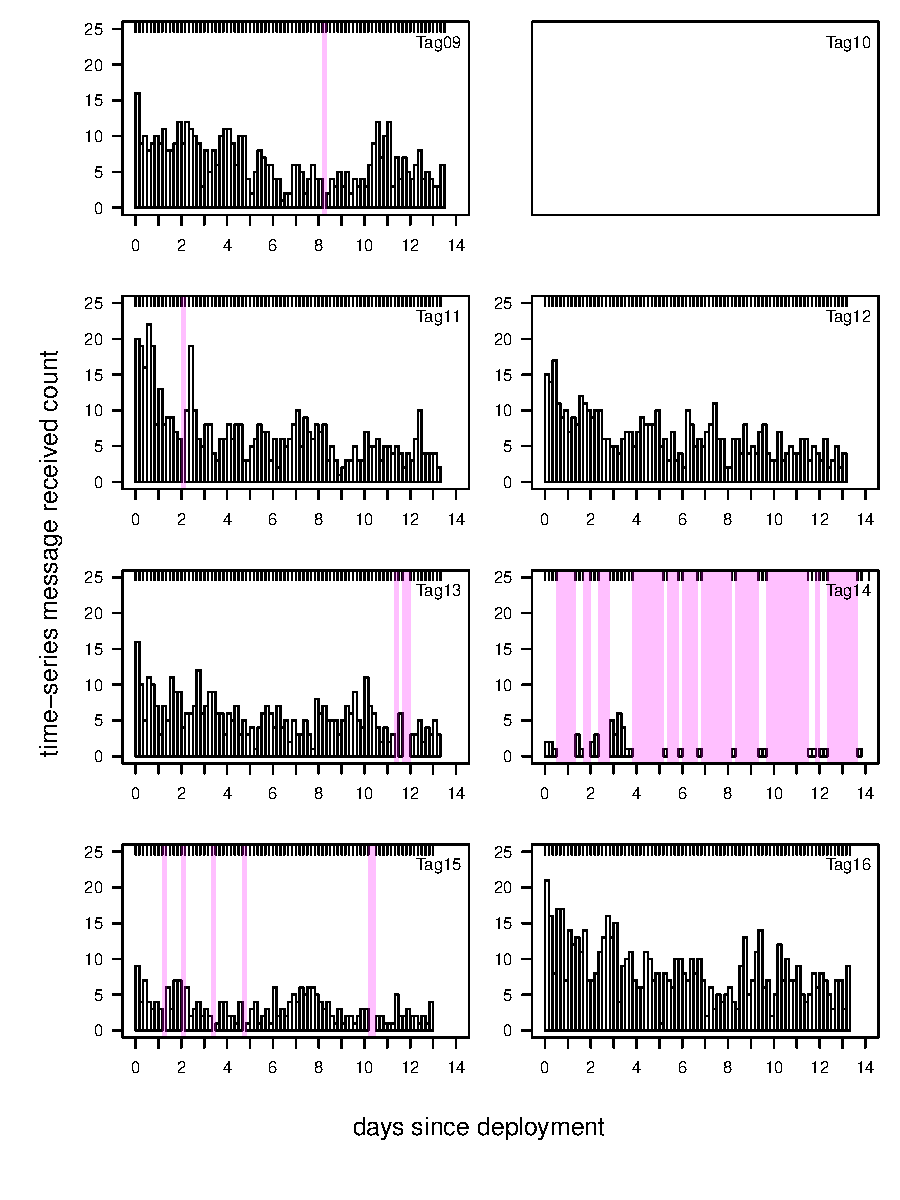
\includegraphics{figure_s1.pdf}
\caption{Time-series message reception count via satellite only for 8 assessment tags in the time-series only programming configuration. Each block represnts 48 time-series data points (at a sampling period of 5 minutes). Blocks are placed at when data was recorded and bar height described the total number of times the message was recieved over the entire life of the tag. Pink bars indicate time periods for which there was a presumed data message generated, but it was never recieved. Malfunctioning tags (Tag13, 14) were truncated to 14 days for comparison purposes.}
\end{figure}

\end{document}
